%%%%%%%%%%%%%%%%%%%%%%%%%%%%%%%%%%%%%%%%%%%%%%%%%%%%%%%%%%%%%%%%%
%
% Project     : Bachelorarbeit
% Title       : Machbarkeitsanalyse für eine ressourcenorientierte Schnittstelle zur Verarbeitung grundlegender Probleme der Informatik
% File        : abstract.tex Rev. 01
% Date        : 01.03.2015
% Author      : Raffael Santschi
%
%%%%%%%%%%%%%%%%%%%%%%%%%%%%%%%%%%%%%%%%%%%%%%%%%%%%%%%%%%%%%%%%%

\chapter{Anhang}\label{chap.anhang}

\section{Risikoanalyse des Projekts}\label{risikoanalyse}
Jedes Projekt birgt Risiken. Werden diese nicht am Anfang analysiert und über die gesamte Projektlaufzeit überwacht, kann es zu grossen Schwierigkeiten kommen. Die angewandten Methoden sind aus \cite{proj_mgmt_book} und aus dem dem Management Fach Projekt und Prozessmanagement bekannt.

\subsection{Risikoermittlung}\label{risikoermittlung}
Die Risikoermittlung wird zur Bestimmung und Folgenabschätzung möglicher Risiken angewendet.

\begin{table}[ht]
\centering
  \begin{tabular}{  p{5cm} | p{9cm} }
	\hline
	\rowcolor{gray}
	\textbf{Risiko}					&	\textbf{Mögliche Folgen}	\\ \hline
	Implementationsschwierigkeiten			&	\begin{itemize}
										\item Zeitplan nicht einhaltbar
										\item Einige Anforderungen müssen zurückgestellt werden
										\item Projektarbeit kann nicht durchgeführt werden
									\end{itemize}	\\ \hline
	Zeitengpässe
								&	\begin{itemize}
										\item Zeitplan nicht einhaltbar
										\item Einige Anforderungen müssen zurückgestellt werden
										\item Projektarbeit kann nicht durchgeführt werden
									\end{itemize}	\\ \hline
	Mangelhaftes Endprodukt		
								&	\begin{itemize}
										\item Produkt muss überarbeitet werden, da keine Abnahme durch den Stakeholder erfolgt
									\end{itemize}	\\ \hline	
	Anforderungen nicht vollständig	
								&	\begin{itemize}
										\item Wichtige Funktionen stehen den Benutzern nicht zur Verfügung
									\end{itemize}	\\ \hline			
  \end{tabular}
   \caption{Risikoermittlung}
\end{table}

\subsection{Risikobewertung}
Das Schadensausmass und die Eintrittswahrscheinlichkeit der Risiken sind nach folgendem Schema bewertet worden:

\begin{table}[ht]
\centering
  \begin{tabular}{ l | p{5cm} | p{5cm} }
	\hline
	\rowcolor{gray}
	\textbf{Wert}					&	\textbf{Eintrittswahrscheinlichkeit} &	\textbf{Schadensausmass}	\\ \hline			
	1							&	sehr unwahrscheinlich		&	vernachlässigbar	\\ \hline
	2							&	unwahrscheinlich			&	spürbar		\\ \hline
	3							&	wenig wahrscheinlich		&	verkraftbar		\\ \hline
	4							&	ziemlich wahrscheinlich		&	gefährlich		\\ \hline
	5							&	sehr wahrscheinlich			&	katastrophal		\\ \hline
  \end{tabular}
   \caption{Risikobewertungsschema}
\end{table}

\FloatBarrier
Die Risiken aus der Risikobewertung (siehe \ref{risikoermittlung}) wurden anhand dieses Schemas bewertet.

\begin{equation*}
Risikofaktor = Eintrittswahrscheinlichkeit * Schadensausmass
\end{equation*}

\begin{table}[ht]
\centering
  \begin{tabular}{ l | p{3cm} | p{3cm} | c }
	\hline
	\rowcolor{gray}
	\textbf{Risiko}					&	\textbf{Eintrittswahr- scheinlichkeit} &	\textbf{Schadensausmass} 	&	\textbf{Risikofaktor}\\ \hline			
	Implementationsschwierigkeiten			&	3					&	4			&	\textbf{12}	\\ \hline
	Zeitengpässe					&	2					&	5			&	\textbf{10}	\\ \hline
	Mangelhaftes Endprodukt				&	2					&	4			&	\textbf{8}	\\ \hline
	Anforderungen nicht vollständig			&	2					&	2			&	4		\\ \hline
  \end{tabular}
   \caption{Risikobewertung}
\end{table}

\subsection{Risikomatrix}
Anhand der Risikobeurteilung konnten die Risiken in eine Risikomatrix eingesetzt werden. Diese Matrix bietet einen guten Überblick über die Risiken und zeigt schnell, welche Risiken beachtet werden müssen.
\begin{figure}[h]
\centering
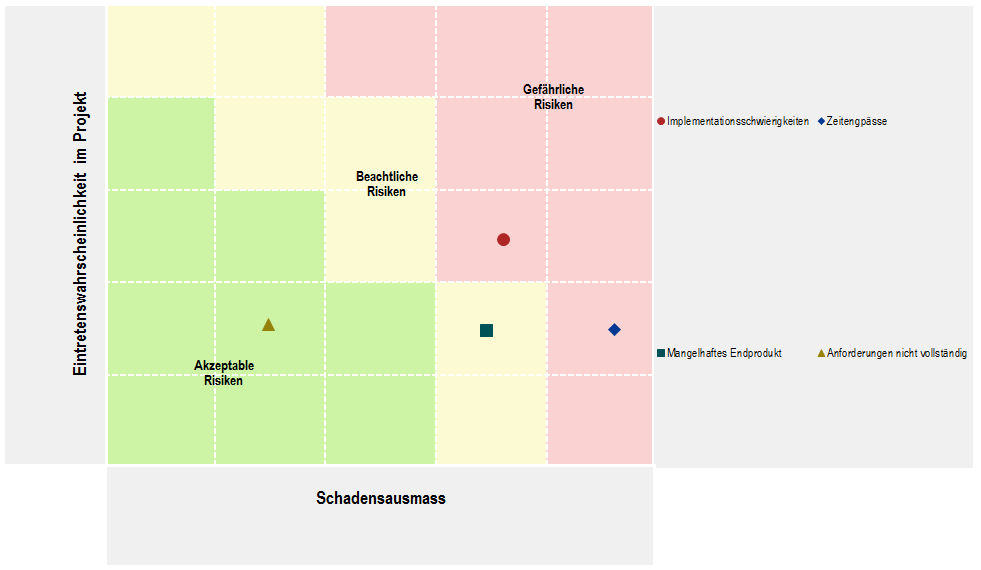
\includegraphics[scale=0.5]{images/excel/risikomatrix.png}
\caption{Risikomatrix}
\label{fig:risikomatrix}
\end{figure}

\subsection{Massnahmen}
Es wurden Massnahmen für die gefundenen Risiken gesucht und festgehalten. Die Massnahmen sind wiederum in vorbeugende Massnahmen und Eventualmassnahmen unterteilt.

\begin{table}[ht]
\centering
  \begin{tabular}{  l | p{4.5cm} | p{4.5cm} }
	\hline
	\rowcolor{darkgray}
	\textbf{Risiko}					&	\multicolumn{2}{|c|}{\textbf{Massnahmen}} \\ \hline
	\rowcolor{gray}
								&	Vorbeugende Massnahmen & Eventualmassnahmen	\\ \hline
	Implementationsschwierigkeiten
								&	\begin{itemize}
										\item Im Zeitplan genügen Reserver einrechnen
										\item Kontaktpersonen zum Thema suchen
										\item Zeitplan einhalten, pünktlich mit den Arbeiten beginnen
									\end{itemize}
								&	\begin{itemize}
										\item Betreuer / Schulleitung informieren
										\item Verschiebungsgesuch stellen
									\end{itemize}						\\ \hline
	Zeitengpässe
								&	\begin{itemize}
										\item Fixe Zeiten einplanen
										\item Tätigkeiten priorisieren
									\end{itemize}
								&	\begin{itemize}
										\item Vorgezogene Präsentation verschieben
										\item Verschiebungsgesuch stellen
									\end{itemize}	\\ \hline
	Mangelhaftes Endprodukt		
								&	\begin{itemize}
										\item Anforderungskatalog sauber erstellen
										\item Kunden laufend über den Stand des Produktes informieren
									\end{itemize}
								&	\begin{itemize}
										\item Lösung mit dem Kunden suchen
										\item Projekt verlängern
									\end{itemize}	\\ \hline	
	Anforderungen nicht vollständig	
								&	\begin{itemize}
										\item Review des Anforderungskataloges
										\item Kunden laufend über den Stand des Produktes informieren
									\end{itemize}
								&	\begin{itemize}
										\item Anforderungen werden aufgenommen und in einen nächsten Release geplant							
									\end{itemize}	\\ \hline			
  \end{tabular}
   \caption{Risikoanalyse - Massnahmen}
\end{table}

\clearpage
\newpage

\section{Schnittstellen Dokumentation}\label{api_doc}

Die Beispiele sind in \gls{json}, es ist jedoch auch sehr einfach möglich die Schnittstelle für \gls{xml}, \gls{yaml} oder andere Formate zu erweitern

%%%%%%%%%%%%%%%%%%%%%%%%%%%%%%%
%
%
%		Rucksack
%
%
%%%%%%%%%%%%%%%%%%%%%%%%%%%%%%%

\subsection{Rucksack}

\paragraph{POST /optimalPackComputations} - Erstellung einer neuen Rucksack Berechnung\mbox{}\\
Erstellt eine neue Berechnung des Rucksack Problems und speichert sie in die Datenbank.\\
\textbf{Status Codes:}\\
200 - OK: Berechnung wurde erstellt, zusätzlich erhält der Nutzer noch die ID der Berechnung.\\
400 - Bad Request: Die Validierung der Eingabedaten ist fehlgeschlagen.\\

\begin{lstlisting}[language=JSON, caption=Beispiel einer Eingabe für das Rucksack Problem, label=lst:input_knapsack]  
{
  "name": "<Berechnungsname>",
  "maxWeight": <Gewichtsschranke>,
  "items": [
    {
      "id": "<Objekt ID (optional)>",
      "name": "<Objekt Name>",
      "weight": <Gewicht>,
      "profit": <Profit>,
      "count": <Anzahl (optional)>
    }
  ]
}
\end{lstlisting}

\paragraph{GET /algorithm/knapsackComputations/\{ID\}} - Abrufen der Eingabedaten einer Rucksack Berechnung\mbox{}\\
Ruft die Eingabedaten einer bestimmten Berechnung des Rucksack Problems ab. Die Daten werden in der Schnittstelle zuerst für den Algorithmus umgewandelt.\\
\textbf{Status Codes:}\\
200 - OK: Die Eingabedaten wurden gefunden und zurückgeben.\\
404 - Not Found: Die Eingabedaten wurden nicht gefunden.\\

\begin{lstlisting}[language=JSON, caption=Beispiel für Eingabedaten des Rucksack Problems für den Algorithmus, label=lst:input_knapsack_algo]  
{
  "id": "<Berechnung ID>",
  "maxWeight": <Gewichtsschranke>,
  "items": [
    {
      "id": "<Objekt ID>",
      "weight": <Gewicht>,
      "profit": <Profit>
    }
  ]
}
\end{lstlisting}

\paragraph{POST /algorithm/knapsackComputations/\{ID\}/solutions} - Speichern einer Lösung für eine Rucksack Berechnung\mbox{}\\
Speichert eine mögliche Lösung für eine Berechnung des Rucksack Problems. Die Lösung wird zuerst für den Nutzer umgewandelt und danach noch validiert.\\
\textbf{Status Codes:}\\
200 - OK: Lösung wurde gespeichert.\\
400 - Bad Request: Die Validierung der Lösung zeigt Fehler auf, zusätzlich werden die Validierungsfehler mitgegeben.\\

\begin{lstlisting}[language=JSON, caption=Beispiel eines Resultates für das Rucksack Problem aus Algorithmus-Sicht, label=lst:solution_knapsack_algo]  
{
  "solutionType": "<Resultat Typ (PARTIAL | FINAL)>",
  "fitness": <Profit des Resultates>,
  "items": [<Liste der Boolean-Werte>]
}
\end{lstlisting}

\paragraph{GET /optimalPackComputations/\{ID\}} - Abrufen des Status einer Rucksack Berechnung\mbox{}\\
Ruft den Status und die Endresultate einer bestimmten Berechnung des Rucksack Problems ab, die Daten werden direkt aus der Datenbank genommen, da sie dort in Nutzer-Sicht abgespeichert sind.\\
\textbf{Status Codes:}\\
200 - OK: Das Endresultat wurden gefunden und zurückgeben.\\
404 - Not Found: Keine Berechnung gefunden.\\

\begin{lstlisting}[language=JSON, caption=Beispiel eines Endresultates für das Rucksack Problem, label=lst:solution_knapsack]  
{
  "computationId": "<Berechnung ID>",
  "profit": <Profit des Resultates>,
  "items": [
    {
      "id": "<Objekt ID>",
      "name": "<Objekt Name>",
      "weight": <Gewicht>,
      "profit": <Profit>,
      "count": <Anzahl>
    }
  ]
}
\end{lstlisting}

%%%%%%%%%%%%%%%%%%%%%%%%%%%%%%%
%
%
%		Knotenfärbung
%
%
%%%%%%%%%%%%%%%%%%%%%%%%%%%%%%%

\subsection{Knotenfärbung}

\paragraph{POST /avoidCollisionComputations} - Erstellung einer neue Knotenfärbungsberechnung\mbox{}\\
Erstellt eine neue Berechnung des Knotenfärbungsproblems und speichert sie in die Datenbank.\\
\textbf{Status Codes:}\\
200 - OK: Berechnung wurde erstellt, zusätzlich erhält der Nutzer noch die ID der Berechnung.\\
400 - Bad Request: Die Validierung der Eingabedaten ist fehlgeschlagen.\\

\begin{lstlisting}[language=JSON, caption=Beispiel einer Eingabe für das Knotenfärbungsproblem, label=lst:input_graphcoloring]  
{
  "name": "<Berechnungsname>",
  "items": [
    {
      "id": "<Element ID (optional)>",
      "name": "<Element Name>",
      "neighbors": [<Benachbarte Elemente>]
    }
  ],
  "possibleValues": [<Moegliche Werte>]
}
\end{lstlisting}

\paragraph{GET /algorithm/graphColoringComputations/\{ID\}} - Abrufen der Eingabedaten einer Knotenfärbungsberechnung\mbox{}\\
Ruft die Eingabedaten einer bestimmten Berechnung des Knotenfärbungsproblems ab. Die Daten werden in der Schnittstelle zuerst für den Algorithmus umgewandelt.\\
\textbf{Status Codes:}\\
200 - OK: Die Eingabedaten wurden gefunden und zurückgeben.\\
404 - Not Found: Die Eingabedaten wurden nicht gefunden.\\

\begin{lstlisting}[language=JSON, caption=Beispiel für Eingabedaten des Knotenfärbungsproblems für den Algorithmus, label=lst:input_graphcoloring_algo]  
{
  "id": "<Berechnung ID>",
  "items": [
    {
      "id": "<Element ID>",
      "neighbors": [<Benachbarte Elemente>]
    }
  ]
}
\end{lstlisting}

\paragraph{POST /algorithm/graphColoringComputations/\{ID\}/solutions} - Speichern einer Lösung für eine Knotenfärbungsberechnung\mbox{}\\
Speichert eine mögliche Lösung für eine Berechnung des Knotenfärbungsproblems. Die Lösung wird zuerst für den Nutzer umgewandelt und danach noch validiert.\\
\textbf{Status Codes:}\\
200 - OK: Lösung wurde gespeichert.\\
400 - Bad Request: Die Validierung der Lösung zeigt Fehler auf, zusätzlich werden die Validierungsfehler mitgegeben.\\

\begin{lstlisting}[language=JSON, caption=Beispiel eines Resultates für das Knotenfärbungsproblems aus Algorithmus-Sicht, label=lst:solution_graphcoloring_algo]  
{
  "solutionType": "<Resultat Typ (PARTIAL | FINAL)>",
  "differentValues": <Anzahl verschiedene Werte>,
  "items": [
    {
      "id": "<Element name>",
      "value": "<Zugewiesener Wert>"
    }
  ]
}
\end{lstlisting}

\paragraph{GET /optimalPackComputations/\{ID\}} - Abrufen des Status einer Rucksack Berechnung\mbox{}\\
Ruft den Status und die Endresultate einer bestimmten Berechnung des Knotenfärbungsproblems ab, die Daten werden direkt aus der Datenbank genommen, da sie dort in Nutzer-Sicht abgespeichert sind.\\
\textbf{Status Codes:}\\
200 - OK: Das Endresultat wurden gefunden und zurückgeben.\\
404 - Not Found: Keine Berechnung gefunden.\\

\begin{lstlisting}[language=JSON, caption=Beispiel eines Endresultates für das Knotenfärbungsproblems, label=lst:solution_graphcoloring]  
{
  "computationId": "<Berechnung ID>",
  "differentValues": <Anzahl verschiedene Werte>,
  "items": [
    {
      "id": "<Element name>",
      "value": "<Zugewiesener Wert (ersetzt durch angegebene Werte)>"
    }
  ]
}
\end{lstlisting}

%%%%%%%%%%%%%%%%%%%%%%%%%%%%%%%
%
%
%		Problem des Handlungsreisenden
%
%
%%%%%%%%%%%%%%%%%%%%%%%%%%%%%%%

\subsection{Problem des Handlungsreisenden}

\paragraph{POST /shortestRouteComputations} - Erstellung einer neue Routenberechnung\mbox{}\\
Erstellt eine neue Berechnung des Problem des Handlungsreisenden und speichert sie in die Datenbank.\\
\textbf{Status Codes:}\\
200 - OK: Berechnung wurde erstellt, zusätzlich erhält der Nutzer noch die ID der Berechnung.\\
400 - Bad Request: Die Validierung der Eingabedaten ist fehlgeschlagen.\\

\begin{lstlisting}[language=JSON, caption=Beispiel einer Eingabe für das Problem des Handlungsreisenden, label=lst:input_tsp]  
{
  "name": "<Berechnungsname>",
  "waypoints": [
    {
      "id": "<Wegpunkt ID (optional)>",
      "name": "<Wegpunkt Name>",
      "duration": <Aufenthaltszeit>,
      "wishedArrival": <Gewuenschte Ankunftszeit>
    }
  ],
  "configuration": {
    "startPoint": {
      "id": "<Wegpunkt ID (optional)>",
      "name": "<Wegpunkt Name>"
    },
    "startTime": <Startzeit>,
    "maxArrivalVariance": <Maximale Abweichung bei den Akunftszeiten>
  }
}
\end{lstlisting}

\paragraph{GET /algorithm/tspComputations/\{ID\}} - Abrufen der Eingabedaten einer Routenberechnung\mbox{}\\
Ruft die Eingabedaten einer bestimmten Berechnung des Problem des Handlungsreisenden ab. Die Daten werden in der Schnittstelle zuerst für den Algorithmus umgewandelt.\\
\textbf{Status Codes:}\\
200 - OK: Die Eingabedaten wurden gefunden und zurückgeben.\\
404 - Not Found: Die Eingabedaten wurden nicht gefunden.\\

\begin{lstlisting}[language=JSON, caption=Beispiel für Eingabedaten des Problem des Handlungsreisenden für den Algorithmus, label=lst:input_tsp_algo]  
{
  "id": "<Berechnung ID>",
  "waypoints": [
    {
      "id": "<Wegpunkt ID>",
      "name": "<Wegpunkt Name>",
      "duration": <Aufenthaltszeit>,
      "wishedArrival": <Gewuenschte Ankunftszeit>
    }
  ],
  "configuration": {
    "startPoint": {
      "id": "<Wegpunkt ID>",
      "name": "<Wegpunkt Name>"
    },
    "startTime": <Startzeit>,
    "maxArrivalVariance": <Maximale Abweichung bei den Akunftszeiten>
  }
}
\end{lstlisting}

\paragraph{POST /algorithm/tspComputations/\{ID\}/solutions} - Speichern einer Lösung für eine Routenberechnung\mbox{}\\
Speichert eine mögliche Lösung für eine Berechnung des Problem des Handlungsreisenden. Die Lösung wird zuerst für den Nutzer umgewandelt und danach noch validiert.\\
\textbf{Status Codes:}\\
200 - OK: Lösung wurde gespeichert.\\
400 - Bad Request: Die Validierung der Lösung zeigt Fehler auf, zusätzlich werden die Validierungsfehler mitgegeben.\\

\begin{lstlisting}[language=JSON, caption=Beispiel eines Resultates für das Problem des Handlungsreisenden aus Algorithmus-Sicht, label=lst:solution_tsp_algo]  
{
  "solutionType": "<Resultat Typ (PARTIAL | FINAL)>",
  "totalLength": <Totale Laenge>,
  "waypoints": [
    {
      "name": "<Wegpunkt Name>"
    }
  ]
}
\end{lstlisting}

\paragraph{GET /shortestRouteComputations/\{ID\}} - Abrufen des Status einer Routenberechnung\mbox{}\\
Ruft den Status und die Endresultate einer bestimmten Berechnung des Problem des Handlungsreisenden ab, die Daten werden direkt aus der Datenbank genommen, da sie dort in Nutzer-Sicht abgespeichert sind.\\
\textbf{Status Codes:}\\
200 - OK: Das Endresultat wurden gefunden und zurückgeben.\\
404 - Not Found: Keine Berechnung gefunden.\\

\begin{lstlisting}[language=JSON, caption=Beispiel eines Endresultates für das Problem des Handlungsreisenden, label=lst:solution_tsp]  
{
  "computationId": "<Berechnung ID>",
  "totalLength": <Totale Laenge>,
  "plannedArrival": <Geplante Endankunftszeit>,
  "waypoints": [
    {
      "id": "<Wegpunkt ID>",
      "name": "<Wegpunkt Name>",
      "duration": <Aufenthaltszeit>,
      "wishedArrival": <Gewuenschte Ankunftszeit>,
      "plannedArrival": <Geplante Ankunftszeit>
    }
  ]
}
\end{lstlisting}

%%%%%%%%%%%%%%%%%%%%%%%%%%%%%%%
%
%
%		Briefträgerproblem
%
%
%%%%%%%%%%%%%%%%%%%%%%%%%%%%%%%

\subsection{Briefträgerproblem}

\paragraph{POST /coverAllConnectionComputations} - Erstellung einer neue Routenberechnung\mbox{}\\
Erstellt eine neue Berechnung des Briefträgerproblem und speichert sie in die Datenbank.\\
\textbf{Status Codes:}\\
200 - OK: Berechnung wurde erstellt, zusätzlich erhält der Nutzer noch die ID der Berechnung.\\
400 - Bad Request: Die Validierung der Eingabedaten ist fehlgeschlagen.\\

\begin{lstlisting}[language=JSON, caption=Beispiel einer Eingabe für das Briefträgerproblem, label=lst:input_postman]  
{
  "name": "<Berechnungsname>",
  "items": [
    {
      "id": "<Wegpunkt ID (optional)>",
      "name": "<Wegpunkt Name>",
      "connections": [
        {
          "item": {<Wegpunkt>},
          "length": <Distanz>
        }
      ]
    }
  ],
  "startPoint": {
    "id": "<Wegpunkt ID (optional)>",
    "name": "<Wegpunkt Name>",
    "connections": [
      {
        "item": {<Wegpunkt>},
        "length": <Distanz>
      }
    ]
  }
}
\end{lstlisting}

\paragraph{GET /algorithm/postmanComputations/\{ID\}} - Abrufen der Eingabedaten einer Routenberechnung\mbox{}\\
Ruft die Eingabedaten einer bestimmten Berechnung des Briefträgerproblem ab. Die Daten werden in der Schnittstelle zuerst für den Algorithmus umgewandelt.\\
\textbf{Status Codes:}\\
200 - OK: Die Eingabedaten wurden gefunden und zurückgeben.\\
404 - Not Found: Die Eingabedaten wurden nicht gefunden.\\

\begin{lstlisting}[language=JSON, caption=Beispiel für Eingabedaten des Briefträgerproblems für den Algorithmus, label=lst:input_postman_algo]  
{
  "id": "<Berechnung ID>",
  "items": [
    {
      "id": "<Wegpunkt ID>",
      "name": "<Wegpunkt Name>",
      "connections": [
        {
          "item": {<Wegpunkt>},
          "length": <Distanz>
        }
      ]
    }
  ],
  "startPoint": {
    "id": "<Wegpunkt ID (optional)>",
    "name": "<Wegpunkt Name>",
    "connections": [
      {
        "item": {<Wegpunkt>},
        "length": <Distanz>
      }
    ]
  }
}
\end{lstlisting}

\paragraph{POST /algorithm/postmanComputations/\{ID\}/solutions} - Speichern einer Lösung für eine Routenberechnung\mbox{}\\
Speichert eine mögliche Lösung für eine Berechnung des Briefträgerproblems. Die Lösung wird zuerst für den Nutzer umgewandelt und danach noch validiert.\\
\textbf{Status Codes:}\\
200 - OK: Lösung wurde gespeichert.\\
400 - Bad Request: Die Validierung der Lösung zeigt Fehler auf, zusätzlich werden die Validierungsfehler mitgegeben.\\

\begin{lstlisting}[language=JSON, caption=Beispiel eines Resultates für das Briefträgerproblem aus Algorithmus-Sicht, label=lst:solution_postman_algo]  
{
  "solutionType": "<Resultat Typ (PARTIAL | FINAL)>",
  "items": [
    {
      "id": "<Wegpunkt ID>"
    }
  ]
}
\end{lstlisting}

\paragraph{GET /coverAllConnectionComputations/\{ID\}} - Abrufen des Status einer Routenberechnung\mbox{}\\
Ruft den Status und die Endresultate einer bestimmten Berechnung des Briefträgerproblems ab, die Daten werden direkt aus der Datenbank genommen, da sie dort in Nutzer-Sicht abgespeichert sind.\\
\textbf{Status Codes:}\\
200 - OK: Das Endresultat wurden gefunden und zurückgeben.\\
404 - Not Found: Keine Berechnung gefunden.\\

\begin{lstlisting}[language=JSON, caption=Beispiel eines Endresultates für das Briefträgerproblem, label=lst:solution_postman]  
{
  "computationId": "<Berechnung ID>",
  "items": [
    {
      "id": "<Wegpunkt ID>",
      "name": "<Wegpunkt Name>"
    }
  ],
  "totalLength": <Totale Laenge>
}
\end{lstlisting}

%%%%%%%%%%%%%%%%%%%%%%%%%%%%%%%
%
%
%		Stundenplan Erstellung
%
%
%%%%%%%%%%%%%%%%%%%%%%%%%%%%%%%

\subsection{Stundenplan Erstellung}

\paragraph{POST /timetableComputations} - Erstellung einer neue Stundenplan Berechnung\mbox{}\\
Erstellt eine neue Berechnung des Stundenplanproblems und speichert sie in die Datenbank.\\
\textbf{Status Codes:}\\
200 - OK: Berechnung wurde erstellt, zusätzlich erhält der Nutzer noch die ID der Berechnung.\\
400 - Bad Request: Die Validierung der Eingabedaten ist fehlgeschlagen.\\

\begin{lstlisting}[language=JSON, caption=Beispiel einer Eingabe für das Stundenplanproblem, label=lst:input_timetableScheduling]  
{
  "name": "<Berechnungsname>",
  "schoolClasses": [
    {
      "id": "<ID Klasse>",
      "name": "<Klassename>",
      "schoolSubjects": [
        {
          "id": "<ID Schulfach>"
        }
      ],
      "size": <Groesse der Klasse>
    }
  ],
  "teachers": [
    {
      "id": "<ID Lehrer>",
      "name": "<Name des Lehrers>",
      "skills": [
        {
          "id": "<ID Schulfach>"
        }
      ],
      "associations": [
        {
          "id": "<ID Klasse (optional)>"
        }
      ],
      "freeDays": [
        {
          "<Wochentag>": {
            "from": <Startzeit (optional)>,
            "to": <Endzeit (optional)>,
            "morning": <Am Morgen (optional)>,
            "afternoon": <Am Nachmittag (optional)>,
            "wholeDay": <Ganzer Tag (optional)>
          }
        }
      ]
    }
  ],
  "classRooms": [
    {
      "id": "<ID Klassenzimmer>",
      "name": "<Klassenzimmername>",
      "allowedSkills": [
        {
          "id": "<ID Schulfach (optional)>"
        }
      ],
      "blockedDays": [
        {
          "<Wochentag>": {
            "from": <Startzeit (optional)>,
            "to": <Endzeit (optional)>,
            "morning": <Am Morgen (optional)>,
            "afternoon": <Am Nachmittag (optional)>,
            "wholeDay": <Ganzer Tag (optional)>
          }
        }
      ],
      "capacity": <Fassungsvermoegen>
    }
  ],
  "schoolSubjects": [
    {
      "id": "<ID Schulfach>",
      "name": "<Schulfachname>",
      "explicitLocation": <Explizites Schulzimmer (optional)>
    }
  ],
  "configuration": {
    "breakTimeSliceSize": [<Pausenzeiten>],
    "dayTimeSlots": [
      {
        "<Wochentag>": {
          "from": <Startzeit (optional)>,
          "to": <Endzeit (optional)>,
          "defaultTimes": <Standard Werte (optional)>
        }
      }
    ],
    "lessonDuration": <Lektionsdauer>
  }
}
\end{lstlisting}

\paragraph{GET /algorithm/timetableComputations/\{ID\}} - Abrufen der Eingabedaten einer Stundenplan Berechnung\mbox{}\\
Ruft die Eingabedaten einer bestimmten Berechnung des Stundenplanproblems ab. Die Daten werden in der Schnittstelle zuerst für den Algorithmus umgewandelt.\\
\textbf{Status Codes:}\\
200 - OK: Die Eingabedaten wurden gefunden und zurückgeben.\\
404 - Not Found: Die Eingabedaten wurden nicht gefunden.\\

\begin{lstlisting}[language=JSON, caption=Beispiel für Eingabedaten des Stundenplanproblems für den Algorithmus, label=lst:input_timetableScheduling_algo]  
{
  "id": "<Berechnung ID>",
  "associations": [
    {
      "id": "<ID Klasse>",
      "name": "<Klassename>",
      "schoolSubjects": [
        {
          "id": "<ID Schulfach>"
        }
      ],
      "size": <Groesse der Klasse>
    }
  ],
  "responsibles": [
    {
      "id": "<ID Lehrer>",
      "name": "<Name des Lehrers>",
      "skills": [
        {
          "id": "<ID Schulfach>"
        }
      ],
      "associations": [
        {
          "id": "<ID Klasse>"
        }
      ],
      "freeDays": [
        {
          "<Wochentag>": {
            "from": <Startzeit>,
            "to": <Endzeit>,
            "morning": <Am Morgen>,
            "afternoon": <Am Nachmittag>,
            "wholeDay": <Ganzer Tag>
          }
        }
      ]
    }
  ],
  "places": [
    {
      "id": "<ID Klassenzimmer>",
      "name": "<Klassenzimmername>",
      "allowedSkills": [
        {
          "id": "<ID Schulfach>"
        }
      ],
      "blockedDays": [
        {
          "<Wochentag>": {
            "from": <Startzeit>,
            "to": <Endzeit>,
            "morning": <Am Morgen>,
            "afternoon": <Am Nachmittag>,
            "wholeDay": <Ganzer Tag>
          }
        }
      ],
      "capacity": <Fassungsvermoegen>
    }
  ],
  "skills": [
    {
      "id": "<ID Schulfach>",
      "name": "<Schulfachname>",
      "explicitLocation": <Explizites Schulzimmer>
    }
  ],
  "timeSlices": [
    {
      "number": <Zeitschlitz Nummer>
    }
  ]
}
\end{lstlisting}

\paragraph{POST /algorithm/timetableComputations/\{ID\}/solutions} - Speichern einer Lösung für eine Stundenplan Berechnung\mbox{}\\
Speichert eine mögliche Lösung für eine Berechnung des Stundenplanproblems. Die Lösung wird zuerst für den Nutzer umgewandelt und danach noch validiert.\\
\textbf{Status Codes:}\\
200 - OK: Lösung wurde gespeichert.\\
400 - Bad Request: Die Validierung der Lösung zeigt Fehler auf, zusätzlich werden die Validierungsfehler mitgegeben.\\

\begin{lstlisting}[language=JSON, caption=Beispiel eines Resultates für das Stundenplanproblem aus Algorithmus-Sicht, label=lst:solution_timetableScheduling_algo]  
{
  "solutionType": "<Resultat Typ (PARTIAL | FINAL)>",
  "timeSlices": [
    {
      "timeSlice": {
        "number": <Zeitschlitz Nummer>
      },
      "responsible": {
        "id": "<ID Lehrer>"
      },
      "association": {
        "id": "<ID Schulklasse>"
      },
      "skill": {
        "id": "<ID Schulfach>"
      },
      "place": {
        "id": "<ID Klassenzimmer>"
      }
    }
  ]
}
\end{lstlisting}

\paragraph{GET /timetableScheduleComputations/\{ID\}} - Abrufen des Status einer Stundenplan Berechnung\mbox{}\\
Ruft den Status und die Endresultate einer bestimmten Berechnung des Stundenplanproblems ab, die Daten werden direkt aus der Datenbank genommen, da sie dort in Nutzer-Sicht abgespeichert sind.\\
\textbf{Status Codes:}\\
200 - OK: Das Endresultat wurden gefunden und zurückgeben.\\
404 - Not Found: Keine Berechnung gefunden.\\

\begin{lstlisting}[language=JSON, caption=Beispiel eines Endresultates für das Stundenplanproblem, label=lst:solution_timetableScheduling]  
{
  "computationId": "<Berechnung ID>",
  "plan": [
    {
      "<Wochentag>": [
        {
          "timeSlice": {
            "from": <Startzeit>,
            "to": <Endzeit>
          },
          "teacher": {
            "id": "<ID Lehrer>",
            "name": "<Name des Lehrers>",
          },
          "schoolClass": {
            "id": "<ID Klasse>",
            "name": "<Klassenname>",
          },
          "schoolSubject": {
            "id": "<ID Schulfach>",
            "name": "<Schulfachname>",
          },
          "classRoom": {
            "id": "<ID Klassenzimmer>",
            "name": "<Klassenzimmername>",
          }
        }
      ]
    }
  ],
  "teacherStatistics": [
    {
      "name": "<Lehrername>",
      "statisticMap": [
        {
          "<Schulfach>": <Anzahl Stunden>
        }
      ]
    }
  ]
}
\end{lstlisting}

%%%%%%%%%%%%%%%%%%%%%%%%%%%%%%%
%
%
%		Spielplan Erstellung
%
%
%%%%%%%%%%%%%%%%%%%%%%%%%%%%%%%

\subsection{Spielplan Erstellung}

\paragraph{POST /matchScheduleComputations} - Erstellung einer neue Spielplan Berechnung\mbox{}\\
Erstellt eine neue Berechnung des Spielplanproblems und speichert sie in die Datenbank.\\
\textbf{Status Codes:}\\
200 - OK: Berechnung wurde erstellt, zusätzlich erhält der Nutzer noch die ID der Berechnung.\\
400 - Bad Request: Die Validierung der Eingabedaten ist fehlgeschlagen.\\

\begin{lstlisting}[language=JSON, caption=Beispiel einer Eingabe für das Spielplanproblem, label=lst:input_matchScheduling]  
{
  "name": "<Berechnungsname>",
  "teams": [
    {
      "id": "<ID Team>",
      "name": "<Teamname>",
      "category": {
          "id": "<ID Kategorie>"
      }
    }
  ],
  "referees": [
    {
      "id": "<ID Schiedsrichter>",
      "name": "<Name des Schiedsrichters>",
      "skills": [
        {
          "id": "<ID Kategorie>"
        }
      ],
      "associations": [
        {
          "id": "<ID Team (optional)>"
        }
      ]
    }
  ],
  "fields": [
    {
      "id": "<ID Spielfeld>",
      "name": "<Spielfeldname>",
      "allowedSkills": [
        {
          "id": "<ID Kategorie (optional)>"
        }
      ]
    }
  ],
  "categories": [
    {
      "id": "<ID Kategorie>",
      "name": "<Kategoriename>"
    }
  ],
  "configuration": {
    "breakTimeSliceSize": [<Pausenzeiten>],
    "timeSliceSize": <Spieldauer>
    "startPoint": <Startpunkt>
  }
}
\end{lstlisting}

\paragraph{GET /algorithm/matchScheduleComputations/\{ID\}} - Abrufen der Eingabedaten einer Spielplan Berechnung\mbox{}\\
Ruft die Eingabedaten einer bestimmten Berechnung des Spielplanproblems ab. Die Daten werden in der Schnittstelle zuerst für den Algorithmus umgewandelt.\\
\textbf{Status Codes:}\\
200 - OK: Die Eingabedaten wurden gefunden und zurückgeben.\\
404 - Not Found: Die Eingabedaten wurden nicht gefunden.\\

\begin{lstlisting}[language=JSON, caption=Beispiel für Eingabedaten des Spielplanproblems für den Algorithmus, label=lst:input_matchScheduling_algo]  
{
  "id": "<Berechnung ID>",
  "associations": [
    {
      "id": "<ID Team>",
      "name": "<Teamname>",
      "category": {
          "id": "<ID Kategorie>"
      }
    }
  ],
  "responsibles": [
    {
      "id": "<ID Schiedsrichter>",
      "name": "<Name des Schiedsrichters>",
      "skills": [
        {
          "id": "<ID Kategorie>"
        }
      ],
      "associations": [
        {
          "id": "<ID Team (optional)>"
        }
      ]
    }
  ],
  "places": [
    {
      "id": "<ID Spielfeld>",
      "name": "<Spielfeldname>",
      "allowedSkills": [
        {
          "id": "<ID Kategorie (optional)>"
        }
      ]
    }
  ],
  "skills": [
    {
      "id": "<ID Kategorie>",
      "name": "<Kategoriename>"
    }
  ]
}
\end{lstlisting}

\paragraph{POST /algorithm/matchScheduleComputations/\{ID\}/solutions} - Speichern einer Lösung für eine Spielplan Berechnung\mbox{}\\
Speichert eine mögliche Lösung für eine Berechnung des Spielplanproblems. Die Lösung wird zuerst für den Nutzer umgewandelt und danach noch validiert.\\
\textbf{Status Codes:}\\
200 - OK: Lösung wurde gespeichert.\\
400 - Bad Request: Die Validierung der Lösung zeigt Fehler auf, zusätzlich werden die Validierungsfehler mitgegeben.\\

\begin{lstlisting}[language=JSON, caption=Beispiel eines Resultates für das Spielplanproblem aus Algorithmus-Sicht, label=lst:solution_matchScheduling_algo]  
{
  "solutionType": "<Resultat Typ (PARTIAL | FINAL)>",
  "timeSlices": [
    {
      "timeSlice": {
        "number": <Zeitschlitz Nummer>
      },
      "responsible": {
        "id": "<ID Schiedsrichter>"
      },
      "association": {
        "team1": {
          "id": "<ID Team>"
        },
        "team2": {
          "id": "<ID Team>"
        }
      },
      "place": {
        "id": "<ID Spielfeld>"
      }
    }
  ]
}
\end{lstlisting}

\paragraph{GET /matchScheduleComputations/\{ID\}} - Abrufen des Status einer Spielplan Berechnung\mbox{}\\
Ruft den Status und die Endresultate einer bestimmten Berechnung des Spielplanproblems ab, die Daten werden direkt aus der Datenbank genommen, da sie dort in Nutzer-Sicht abgespeichert sind.\\
\textbf{Status Codes:}\\
200 - OK: Das Endresultat wurden gefunden und zurückgeben.\\
404 - Not Found: Keine Berechnung gefunden.\\

\begin{lstlisting}[language=JSON, caption=Beispiel eines Endresultates für das Spielplanproblem, label=lst:solution_matchScheduling]  
{
  "computationId": "<Berechnung ID>",
  "timeSlices": [
    {
      "timeSlice": {
        "from": <Startzeit>,
        "to": <Endzeit>
      },
      "referee": {
        "id": "<ID Schiedsrichter>",
        "name": "<Name des Schiedsrichters>",
      },
      "teams": {
        "team1": {
          "id": "<ID Team>",
          "name": "<Teamname>",
        },
        "team2": {
          "id": "<ID Team>",
          "name": "<Teamname>",
        }
      },
      "categorie": {
        "id": "<ID Kategorie>",
        "name": "<Kategoriename>",
      },
      "field": {
        "id": "<ID Klassenzimmer>",
        "name": "<Klassenzimmername>",
      }
    }
  ],
  "refereeStatistics": [
    {
      "name": "<Schiedsrichtername>",
      "statisticMap": [
        {
          "<Kategoriename>": <Anzahl Spiele>
        }
      ]
    }
  ],
  "teamStatistics": [
    {
      "name": "<Kategoriename>",
      "statisticMap": [
        {
          "<Teamname>": <Anzahl Spiele>
        }
      ]
    }
  ]
}
\end{lstlisting}